\section{Results}

\subsection{Descriptive statistics}

168,347 patients (with onset-to-scan of within 255 minutes) attended 118 hospitals with total stroke admissions per hospital ranging from 358 to 4,559, and with hospital thrombolysis rates ranging from 5.9\% to 39.2\%. Of the 133,516 patients who did not receive thrombolysis, their range of disability at discharge was: 12\% mRS 0, 33\% mRS 0-1, 52\% mRS 0-2, 69\% mRS 0-3, 82\% mRS 0-4, and 88\% mRS 0-5 at discharge. Of the 34,831 patients who received thrombolysis, their range of disability at discharge was: 15\% mRS 0, 35\% mRS 0-1, 54\% mRS 0-2, 69\% mRS 0-3, 81\% mRS 0-4, and 86\% mRS 0-5. Table \ref{tab:descriptive_stats} shows further descriptive statistics for patients who received or did not receive thrombolysis. Further descriptive statistics are provided in the Supplemental Material.

\begin{minipage}{1\textwidth}
\small
\begin{longtable}[]{@{}l | lll | lll @{}}
\caption{Descriptive statistics for patients receving or not receiving thrombolysis.}\\
\toprule\noalign{}
& \multicolumn{3}{c|}{Thrombolysis given} & \multicolumn{3}{c}{Thrombolysis not given} \\ 
%\midrule\noalign{}
\endhead
\bottomrule\noalign{}
\endlastfoot

& n & Mean (StdDev) & Median (IQR) & n & Mean (StdDev) & Median (IQR) \\
\midrule\noalign{}
Age & 41163 & 72.3 (13.6) & 72.5 (62.5-82.5) & 315941 & 74.5 (13.3) & 77.5 (67.5-82.5) \\
Infarction & 41163 & 1 (NA) & NA & 315941 & 0.86 (NA) & NA \\
Stroke severity & 41163 & 11.0 (7.1) & 9 (5-16) & 315941 & 6.6 (7.6) & 4 (2-8) \\
Prior disability & 41163 & 0.71 (1.17) & 0 (0-1) & 315941 & 1.08 (1.39) & 0 (0-2) \\
Male & 41163 & 0.56 (NA) & NA & 315941 & 0.53 (NA) & NA \\
Onset known & 41163 & 0.99 (NA) & NA & 315941 & 0.63 (NA) & NA \\
Precise onset known & 41163 & 0.80 (NA) & NA & 315941 & 0.28 (NA) & NA \\
Onset during sleep & 41163 & 0.01 (NA) & NA & 315941 & 0.15 (NA) & NA \\
Onset to arrival time & 40583 & 102 (53) & 90 (66-128) & 198105 & 57 (1115) & 250 (112-713) \\
Arrive by ambulance & 41161 & 0.92 (NA) & NA & 315934 & 0.77 (NA) & NA \\
Arrival to scan time & 41163 & 23 (20) & 19 (11-29) & 315941 & 217 (2016) & 61 (26-149) \\
Congestive heart failure & 41163 & 0.04 (NA) & NA & 315941 & 0.05 (NA) & NA \\
Hypertension & 41163 & 0.51 (NA) & NA & 315941 & 0.55 (NA) & NA \\
Atrial fibrillation (Afib) & 41163 & 0.12 (NA) & NA & 315941 & 0.19 (NA) & NA \\
New afib diagnosis & 24485 & 0.11 (NA) & NA & 172727 & 0.06 (NA) & NA \\
Diabetes & 41163 & 0.17 (NA) & NA & 315941 & 0.22 (NA) & NA \\
Prior stroke tia & 41163 & 0.20 (NA) & NA & 315941 & 0.26 (NA) & NA \\
Afib antiplatelet & 41163 & 0.03 (NA) & NA & 315940 & 0.03 (NA) & NA \\
Afib anticoagulant & 30128 & 0.04 (NA) & NA & 237923 & 0.19 (NA) & NA \\
Afib vit k anticoagulant & 41163 & 0.01 (NA) & NA & 315940 & 0.03 (NA) & NA \\
Afib DOAC anticoagulant & 41163 & 0.01 (NA) & NA & 315940 & 0.08 (NA) & NA \\
Afib heparin anticoagulant & 41163 & 0.00 (NA) & NA & 315940 & 0.00 (NA) & NA \\
Thrombolysis & 41163 & 1.00 (NA) & NA & 315941 & 0.00 (NA) & NA \\
Scan to thrombolysis time & 41163 & 37 (29) & 31 (19-47) & NA & NA & NA \\
Thrombectomy & 41163 & 0.06 (NA) & NA & 315941 & 0.01 (NA) & NA \\
Arrival to thrombectomy time & 2591 & 201 (179) & 171 (114-233) & 1752 & 249 (278) & 172 (104-269) \\
\label{tab:descriptive_stats}
\end{longtable}
\end{minipage}

\subsection{Feature selection and proposed causal model}

Features affecting choice of thrombolysis have previously been described \cite{pearn_are_2024}. Details of feature selection for outcome prediction are detailed in the supplementary material. Based also on the selection of characteristics for the prediction of the outcome, we developed figure \ref{fig:dag} as a causal diagram of the factors that affect the use of thrombolysis and the factors that directly affect the outcome. This proposed causal model is based on features identified as affecting outcome or propensity to use thrombolysis, correlations present in the data, known temporal relationships in the data, and clinical review. 

\begin{figure}[!h]
    \centering%\captionsetup{width=.8\linewidth}%
      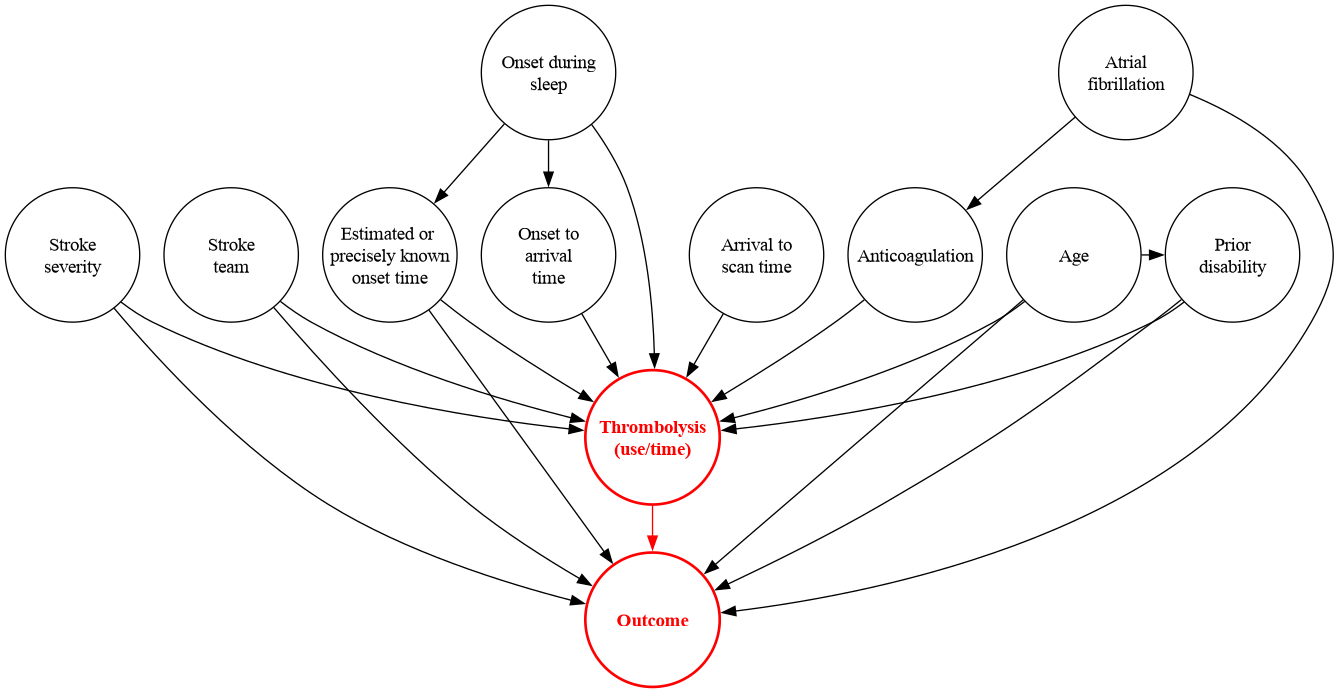
\includegraphics[width=0.95\linewidth]{./images_main/fig_1_thrombolysis_dag.png}\\
  \caption{A Directed Acyclic Graph (`DAG') showing the proposed causal relationships in propensity to use thrombolysis and outcome after stroke with or without thrombolysis.}
    \label{fig:dag}
\end{figure}

\begin{minipage}{1.0\textwidth}

In order to isolate the effect of thrombolysis appropriately, we predicted outcome based on use/time to thrombolysis, and 6 factors identified as confounding variables (affecting both outcome directly and propensity to use thrombolysis).
    
\begin{enumerate}
    \item Onset to thrombolysis time
    \item Prior disability level: mRS before stroke
    \item Stroke severity: NIHSS on arrival
    \item Stroke team: Hospital first attended
    \item Age: As midpoint of 5 year age bands
    \item Atrial fibrillation diagnosis: Patient had a diagnosis of atrial fibrillation either on arrival or diagnosed during admission
    \item Precise onset known: Onset time recorded was recorded as being precise time (as opposed to a best estimate)
\end{enumerate}
\end{minipage}

\subsection{Model accuracy}

With these seven input features, the overall accuracy ranged from 77. 6\% to 89. 7\% in the six mRS disability level models (the standard deviation of accuracy across the 5 k-fold train/test splits ranged from 0.1\% to 0.2\%). This represented between 95-98\% of the accuracy that is obtained with all the features as inputs. ROC-AUC ranged from 0.852 to 0.893 across the six models (standard deviation of the ROC-AUC across the 5 k-folds ranged from 0.001 to 0.002). Results were reproducible across the 5 k-folds, so subsequent analysis was performed on the first k-fold split.

\subsection{SHAP patterns}

SHAP values were calculated for each feature for each patient, showing how each value affects the log odds of achieving a good outcome at discharge. For each patient in the test set we extracted SHAP values for each feature with its corresponding feature value. Figure \ref{fig:shap}a shows the relationship between feature values and the odds of a patient having an excellent outcome (mRS 0-1) at discharge (a positive SHAP value contributes to an increased likelihood, and a negative SHAP value contributes to a reduced likelihood). We found that low prior disability, lower stroke severity, younger age, receiving thrombolysis (and receiving it sooner after onset), and having no diagnosis of atrial fibrillation contributed to a patient more likely having an excellent outcome at discharge. Figure \ref{fig:shap}b focusses on the feature \textit{onset to thrombolysis time}, and its effect on reaching any disability threshold. As time from onset to treatment increased, the beneficial effect of thrombolysis decayed. For thresholds up to, and including, mRS 3, the median effect of thrombolysis remained positive, compared to not receiving thrombolysis, up until the maximum time of 720 minutes. For thresholds of mRS 4 and upwards, the median effect of thrombolysis became negative at longer onset-to-treatment times. This was especially apparent in how thrombolysis changed the overall odds of survival (mRS 0-5) where the median effect of thrombolysis became negative from about 155 minutes. Later thrombolysis may therefore increase the proportion of patients attaining mRS 0-3, but at the cost of some reduction in overall survival. Earlier thrombolysis improved the odds of survival. Figure \ref{fig:shap}c shows the contribution from attending a specific hospital to predicting whether the patient had a good outcome at discharge, for each of the mRS threshold levels used to define a good outcome. As the threshold for having a good outcome becomes more inclusive of higher disability levels, the effect of the hospital attended had a reduced contribution. In other words, the hospital attended made a greater contribution to variation in outcome with thrombolysis for patients with lesser degrees of disability after treatment.


%%%%%%%% PUT ON SEPARATE A4 PAGE LANDSCAPE %%%%%%%%%%%



%\begin{sidewaysfigure}[!ht]
\begin{figure}[!ht]
  \includegraphics[width=1.0\textwidth]{./images_main/fig_2_shap}\\
  \caption{The relationship between feature values and SHAP values in predicting whether a patient will have a good outcome at discharge, for each of the mRS scores used to define a good outcome. Violin plots show the distribution of SHAP values across the patient population for each feature value, with the mid-line showing the median SHAP value.}
  \label{fig:shap}
\end{figure}


\subsection{Counterfactuals - what if patients had not received thrombolysis?}

Using the counterfactual results for all of the patients in the first k-fold test set that received thrombolysis within 300 minutes from stroke onset (n = 6,796), table \ref{tab:stats_table_mrs1} shows a linear regression fitted to the shift in the contribution of thrombolysis towards having an excellent outcome at discharge (mRS 0-1) with respect to the onset to thrombolysis time. We found, for all treated patients, that the effect of thrombolysis had declined to zero at 328 minutes, and the effect from thrombolysis was improving log odds of a good outcome by 0.90 if it were, theoretically, given at the time of stroke onset. We observed that the maximum theoretical effect of thrombolysis (if given at time of stroke onset) was greater for the severe stroke group (1.048 log odds) than the mild-moderate stroke group (0.771 log odds). However the effect of thrombolysis declined more rapidly in the severe stroke group, reaching no effect at 314 minutes for severe stroke patients, compared to 351 minutes for mild-moderate stroke patients. 

\begin{figure}[!ht]
    \centering
    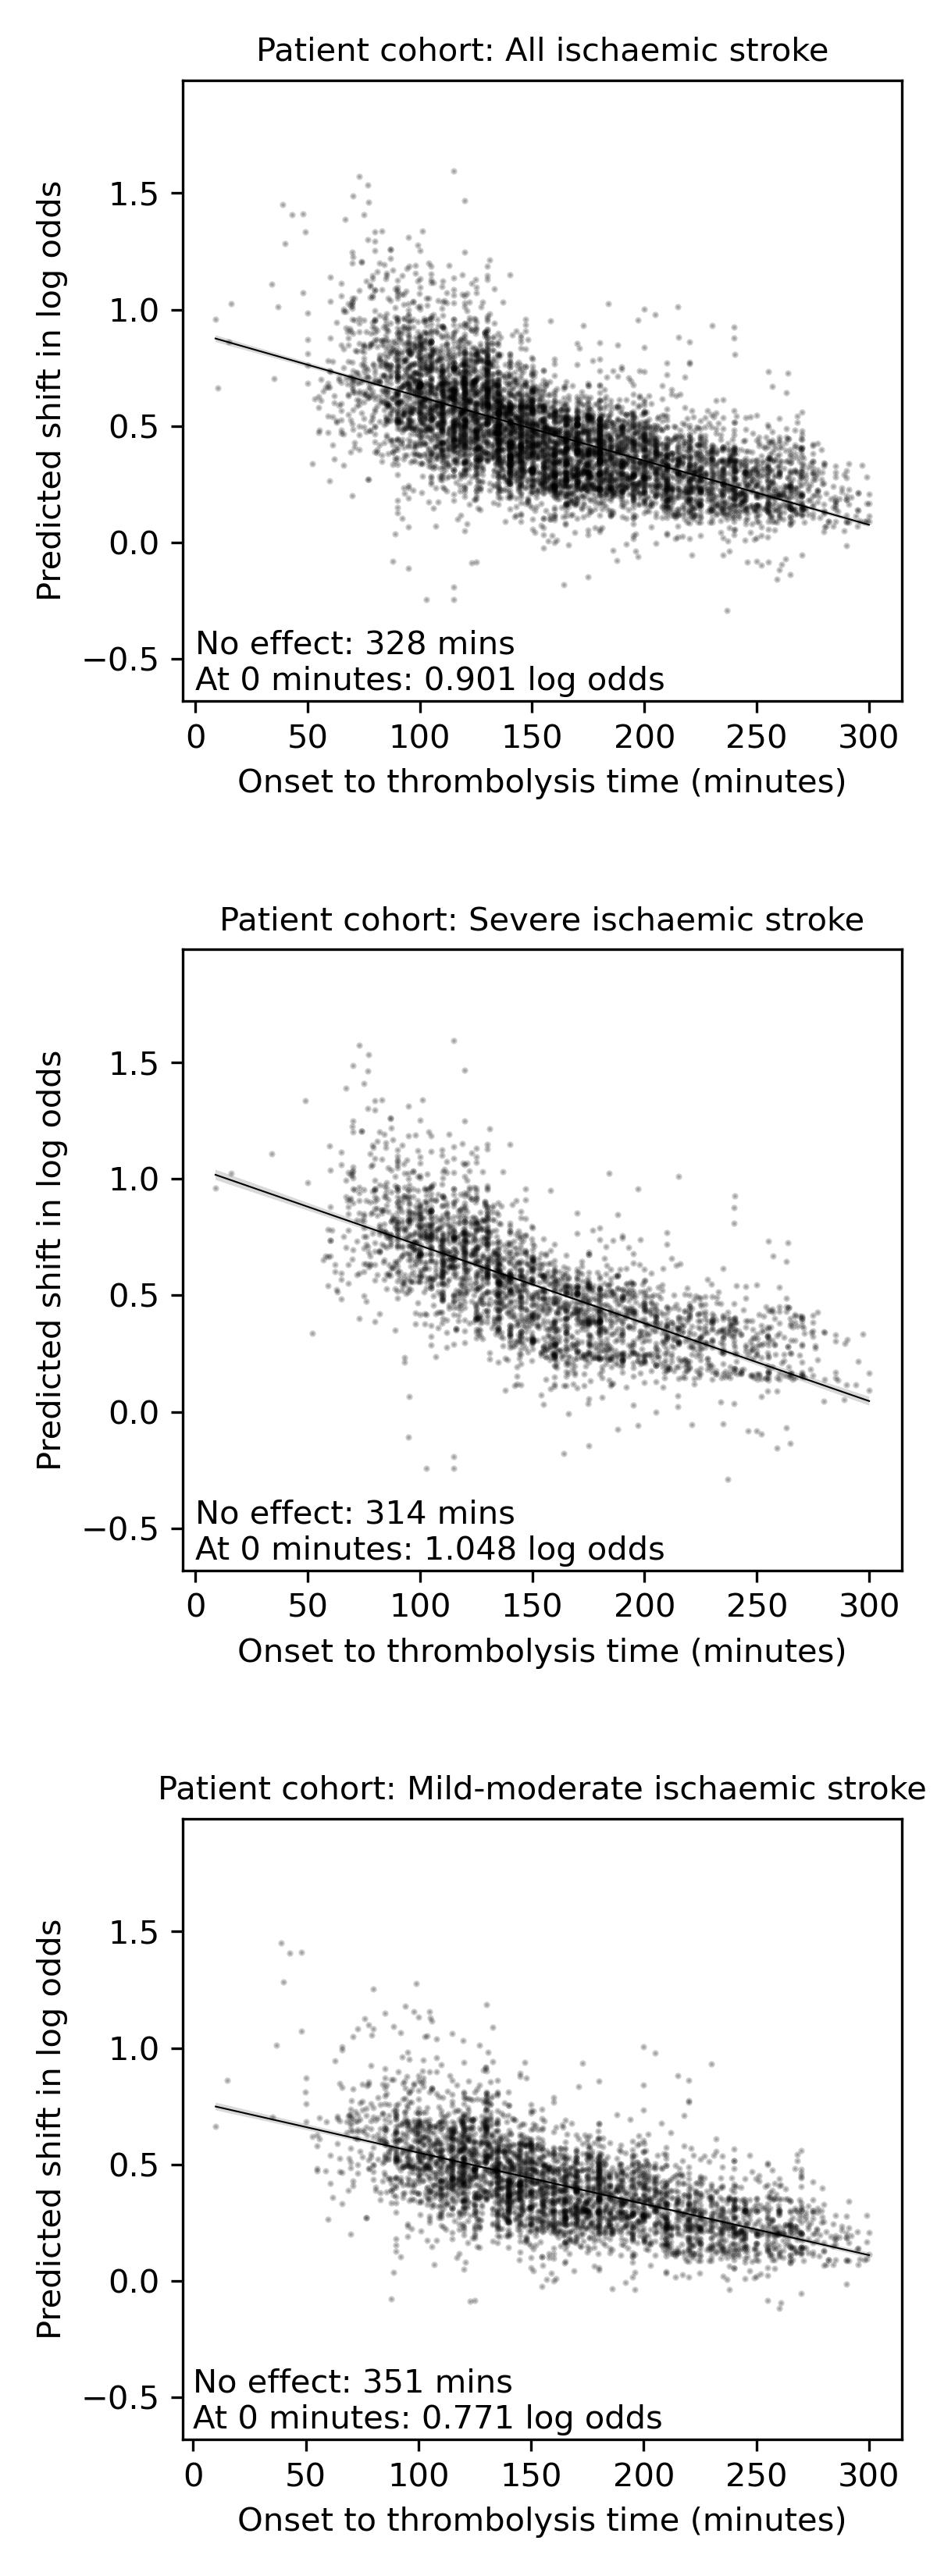
\includegraphics[width=1.0\textwidth]{./images_main/fig_3_linear_reg}\\
    \caption{Linear regression of thrombolysis contribution to excellent outcome (mRS 0–1) at discharge as a function of onset-to-treatment time (OTT) in patients treated within 300 minutes. Left: all treated stroke patients (n = 6,796); Middle: severe stroke patients (NIHSS 11+; n = 2,856); Right: mild-moderate stroke patients (NIHSS 0–10; n = 3,940).}
    \label{fig:linear_regression_plots}
\end{figure}



\begin{table}[!ht]
    \caption{Linear regression of the relationship between onset-to-treatment time (OTT) and the improvement in log-odds of achieving an excellent outcome (mRS 0-1), stratified by stroke severity.}
    \centering
    \begin{tabular}{lllllllll}
    \toprule
    Ischaemic stroke type & Variables & Estimate&  std err & \makecell{Low 95\%\\confidence} & \makecell{High 95\%\\confidence} & t & P$>$$|$t$|$ \\
    \midrule
    All & Constant & 0.901 & 0.007 & 0.888 & 0.915 & 132.5 & 0.000 \\
        & OTT (min) coef & -0.0027 & 4.04e-05 & -0.003 & -0.003 & -68.1 & 0.000 \\
    \midrule
    Severe & Constant & 1.048 & 0.011 & 1.026 & 1.069 & 96.7 & 0.000 \\
    NIHSS 11+ & OTT (mins) coef & -0.0033 & 6.67e-05 & -0.003 & -0.003 & -50.0 & 0.000 \\
    \midrule
    Mild-moderate & Constant & 0.771 & 0.008 & 0.755 & 0.786 & 97.6 & 0.000 \\
    (NIHSS 0-10) & OTT (mins) coef & -0.0022 & 4.57e-05 & -0.002 & -0.002 & -48.1 & 0.000 \\
    \bottomrule
    \end{tabular}
    \label{tab:stats_table_mrs1}
\end{table}


\FloatBarrier
